\documentclass{article}
\usepackage{amsmath, amssymb}
\usepackage{tikz}
\usetikzlibrary{arrows.meta}

\begin{document}

\begin{figure}[h]
    \centering
    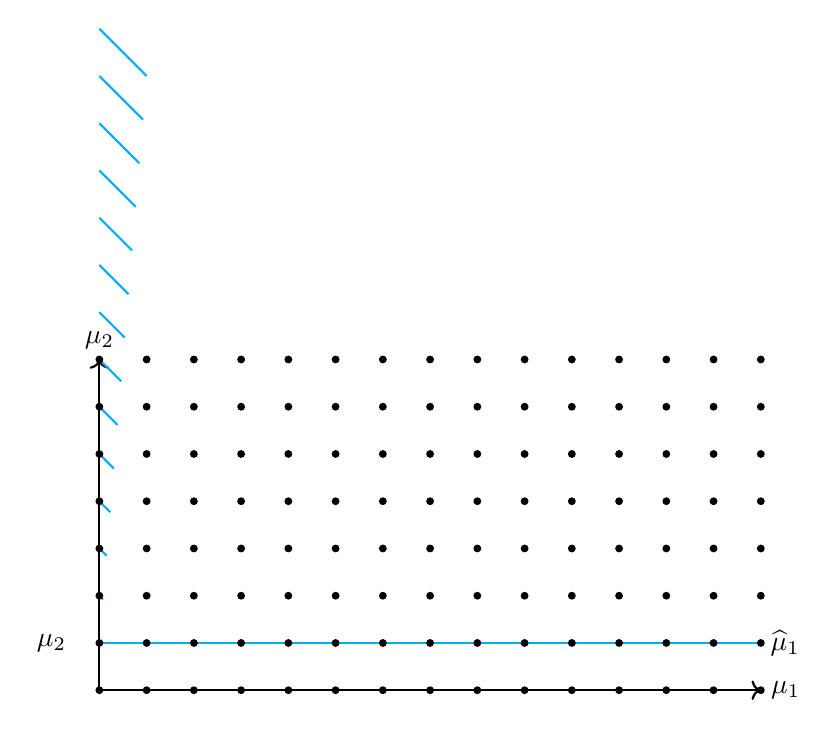
\begin{tikzpicture}[scale=0.6]
        % Axes
        \draw[->, thick] (0,0) -- (14,0) node[right] {$\mu_1$};
        \draw[->, thick] (0,0) -- (0,7) node[above] {$\mu_2$};
        
        % Horizontal line at y=1
        \draw[cyan, thick] (0,1) -- (14,1);
        
        % Diagonal lines representing recurrence
        \foreach \i in {1,...,13}{
            \draw[cyan, thick, domain=0:\i/13] plot (\x,{1+\i-\x});
        }
        
        % Points on the grid
        \foreach \x in {0,...,14}{
            \foreach \y in {0,...,7}{
                \filldraw (\x,\y) circle (2pt);
            }
        }
        
        % Label for horizontal line
        \node at (14, 1) [right] {$\widehat{\mu}_1$};
        
        % Label for diagonal lines
        \node at (-0.5, 1) [left] {$\mu_2$};
    \end{tikzpicture}
    \caption{Recurrence coefficients of $(\mu_1, \mu_2)$ computed via the CC algorithm. On the upper boundary, we find the recurrence coefficients of $\widehat{\mu}_1$.}
    \label{fig:recurrence_coefficients}
\end{figure}

\end{document}